Se le llama caída libre al movimiento de un cuerpo que se debe únicamente a la
influencia de la gravedad (g) y no se toma en cuenta la resistencia del medio en
el que se mueve. Todos los cuerpos con este tipo de movimiento tienen una aceleración dirigida hacia abajo cuyo valor depende de la altura a la que se encuentren. El valor de g en la Tierra es de aproximadamente 9.8 m/s 2 , es decir, los cuerpos
en caída libre (sin considerar la resistencia del aire) aumentan su velocidad (hacia
abajo) en 9.8 m/s cada segundo.\\

La expresión algebraica para calcular la altura h a la que se encontrará un objeto después de un tiempo t de haber sido dejado caer (soltado o impulsado, en
el primer caso la velocidad inicial v 0 es cero y en el segundo es distinto de cero)
desde una altura inicial $h_0$ es:
\begin{equation}\label{eq:caida_libre}
    h=h_0+v_0t-\dfrac{1}{2}gt^2
\end{equation}

Con base en lo anterior,
\begin{multicols}{2}
    \begin{parts}
        ¿a qué altura estará un objeto que se deja caer desde una altura de 182 m después de 6 s?

        \begin{solutionbox}{1.2cm}
        \end{solutionbox}

        Escribe la expresión algebraica considerando las condiciones de inicio. ¿Cuál es la variable dependiente y cuál la independiente?

        \begin{solutionbox}{1.2cm}
        \end{solutionbox}

        Grafica la función (\ref{eq:caida_libre}).

        \begin{figure}[H]
            \centering
            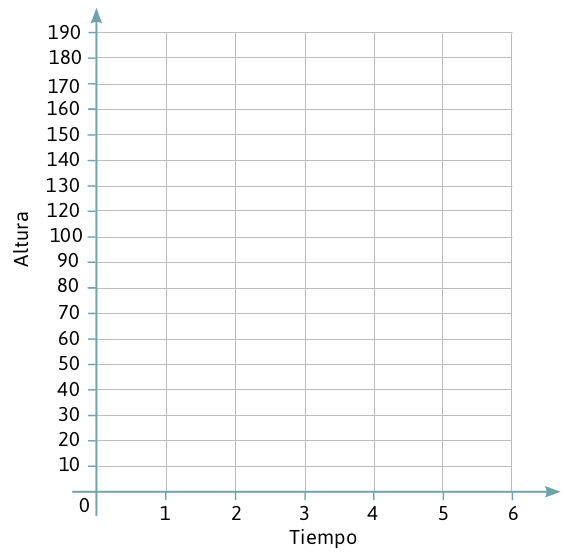
\includegraphics[width=\linewidth]{../images/20230326234935}
            \caption{}
            \label{fig:20230326234935}
        \end{figure}

        \columnbreak
        Completa la Tabla \ref{tab:caida_libre}.

        \begin{table}[H]
            \caption{Tabla con los datos de caida libre}
            \label{tab:caida_libre}
            \begin{tabular}{|*{2}{p{2.5cm}|}}
                \toprule
                Tiempo (s) & Altura (m) \\\hline
                \midrule
                1          &            \\\hline
                1.5        &            \\\hline
                2          &            \\\hline
                2.5        &            \\\hline
                3          &            \\\hline
                3.5        &            \\\hline
                4          &            \\\hline
                4.5        &            \\\hline
                5          &            \\\hline
                5.5        &            \\\hline
                6          &            \\\hline
                           &            \\\hline
                \bottomrule
            \end{tabular}
        \end{table}

        Con base en la tabla, ¿hay dos valores distintos de la variable $t$ que arrojen el mismo valor de h?

        \begin{solutionbox}{1.2cm}
        \end{solutionbox}

        Con base en la gráfica, ¿hay dos valores distintos de la variable $t$ que arrojen el mismo valor de h?

        \begin{solutionbox}{1.2cm}
        \end{solutionbox}

    \end{parts}
\end{multicols}